\documentclass[a4paper]{article}

\usepackage{fullpage} % Package to use full page
\usepackage{parskip} % Package to tweak paragraph skipping
\usepackage{tikz} % Package for drawing
\usepackage{amsmath}
\usepackage{hyperref}
\usepackage{enumitem}
\usepackage{mathtools}
\usepackage{graphicx}
\usepackage{listings}

\title{Scalable Machine Learning - Review Questions 6}
\author{TheBrightSideOfLife: Giorgio Ruffa - Erik Wouters}
\date{11/12/2018}

\begin{document}

\maketitle

\url{https://id2223kth.github.io/slides/questions6.pdf}

\section{CNN Parameters}

The size of the input and padding strategy does not affect the number of parameters (weights) in the model, as the kernels slide on the image.

If a kernel has dimensions $m * n$ and his input has a depth of $l$ channels, for each kernel we will have $m * n * l$ weights, since we have a $m * n$ different set of weights for each input channel (see \cite{cnntutorial} section "Convolution Demo").
If each layer has $k$ kernels (which will create $k$ feature maps as an input of the next layer) and we consider one bias term per kernel, we obtain as a total number of parameters for the layer $i$:
\begin{equation}
    tot_{i} = (n_{i} * m_{i} * l_{i} + 1) * k_{i} 
\end{equation}

In our case, we will have

\begin{equation*}
\begin{split}
    tot_{1} &= (n_{1} m_{1} l_{1} + 1) k_{1} = (3 \times 3  \times 3 + 1 ) \times 100 = 2800 \\
    tot_{2} &= (n_{2} m_{2} k_{1} + 1) k_{2} = (3 \times 3  \times 100 + 1 ) \times 200 = 180200  \\
    tot_{3} &= (n_{3} m_{3} k_{2} + 1) k_{3} = (3 \times 3  \times 200 + 1 ) \times 400 = 720400 \\
\end{split}    
\end{equation*}
hence
\begin{equation*}
\begin{split}
    tot = 2800 + 180200 + 720400 = 903400
\end{split}    
\end{equation*}




\section{CNN filter}
If we apply the filter on the right of figure \ref{fig:q2} to the image on the left using a stride of $2$ in both the $x$ and $y$ directions we get the filtered image in \ref{mat:ans}.

\begin{figure}[ht]
  \centering
  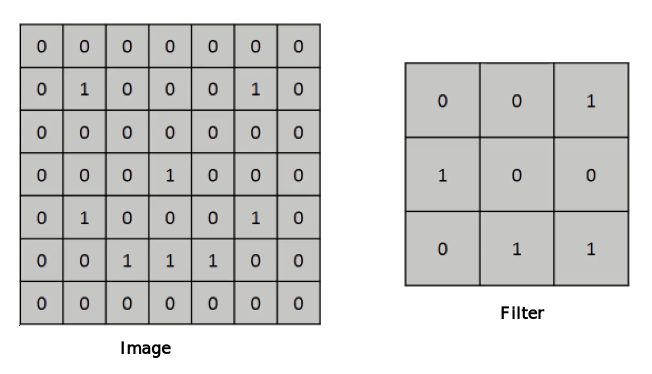
\includegraphics[scale=0.4]{Reports/Images/q2.png}
  \caption{Image and Filter}
  \label{fig:q2}
\end{figure}

\begin{align}
\begin{bmatrix}
     0              & 0             & 0             \\
     \frac{1}{9}    & 0             & \frac{1}{9}   \\
     0              & \frac{1}{9}   & \frac{1}{9}   \\
 \end{bmatrix}
 \label{mat:ans}
\end{align}
Note that the normalization factor may be omitted in case of deep learning applications.

The following Python code snipped can be used to compute the result of the filter:

\begin{lstlisting}[language=Python]
def cf(im, filt, stride=1):
    nx = int(np.ceil((im.shape[0] - filt.shape[0] + 1) / stride))
    ny = int(np.ceil((im.shape[1] - filt.shape[1] + 1) / stride))
    image = np.zeros(shape=(nx, ny))
    for x in range(nx):
        for y in range(ny):
            image[x, y] = np.sum(
                im[
                    x * stride : x * stride + filt.shape[0],
                    y * stride : y * stride + filt.shape[1],
                ]
                * filt
            )
    return image / np.prod(filt.shape)
\end{lstlisting}


\section{Accuracy}
It is not clear to us what does "correlation between kernels" means, as kernels in the same layer are independent between each others. Nevertheless, as shown in the first question, the number of parameters in mainly influenced by the number of kernels, so this increase in number of kernels makes the number of parameters explode, giving rise to overfitting. We are more incline to consider answer (\textit{c}) to be the correct one. Another possible explanation is that if the number of kernels is high compared to the variance of the input image, they may converge to similar values during training, hence overfit the data.
% The correct answer is (c). When the number of kernels increases above a certain limit (which depends on the variance of the input image) the correlation between the kernels starts to increase. This does indeed help the model to overfit the data.

% \bibliography{bibliography}{}
% \bibliographystyle{plain}
\bibliography{bibliography}{}
\bibliographystyle{plain}

\end{document}